\documentclass[12pt]{article}
\usepackage{latexblog}

% ============================================================
% Blog Metadata
% ============================================================
\blogtitle{Redis Memory limit and eviction policy configuration}
\blogdate{2020-03-10}
\blogtags{Redis, 闲话编程, 存储}
\bloglang{en}
\blogsummary{}

\begin{document}
\makeblogtitle

By default, the redis running inside docker has no limitation about memory however generally the container has. Thus if no further configuation of eviction or memory limit is set in redis, you may possibly get some error like Out-of-memory if you keep adding new keys to redis.

\section{Testing with docker}\label{testing-with-docker}

\subsection{Create a simple application}\label{create-a-simple-application}

To reproduce the problem, let's create a simple application by using SpringBoot. We'll have a post api for generating a random item and insert it into redis:

\begin{Shaded}
\begin{Highlighting}[]
\AttributeTok{@PostMapping}\OperatorTok{(}\StringTok{"/generate"}\OperatorTok{)}
\KeywordTok{public}\NormalTok{ Item }\FunctionTok{generate}\OperatorTok{()} \OperatorTok{\{}
\NormalTok{  Item item }\OperatorTok{=}\NormalTok{ Item}\OperatorTok{.}\FunctionTok{random}\OperatorTok{();}
\NormalTok{  redisTemplate}\OperatorTok{.}\FunctionTok{opsForValue}\OperatorTok{().}\FunctionTok{set}\OperatorTok{(}\NormalTok{item}\OperatorTok{.}\FunctionTok{getId}\OperatorTok{(),}\NormalTok{ item}\OperatorTok{);}
  \ControlFlowTok{return}\NormalTok{ item}\OperatorTok{;}
\OperatorTok{\}}
\end{Highlighting}
\end{Shaded}

\subsection{Keep inserting data via jmeter}\label{keep-inserting-data-via-jmeter}

In order to keep inserting data into redis using the post api, we can use Apache jmeter to do this job.

\begin{figure}
\centering
\pandocbounded{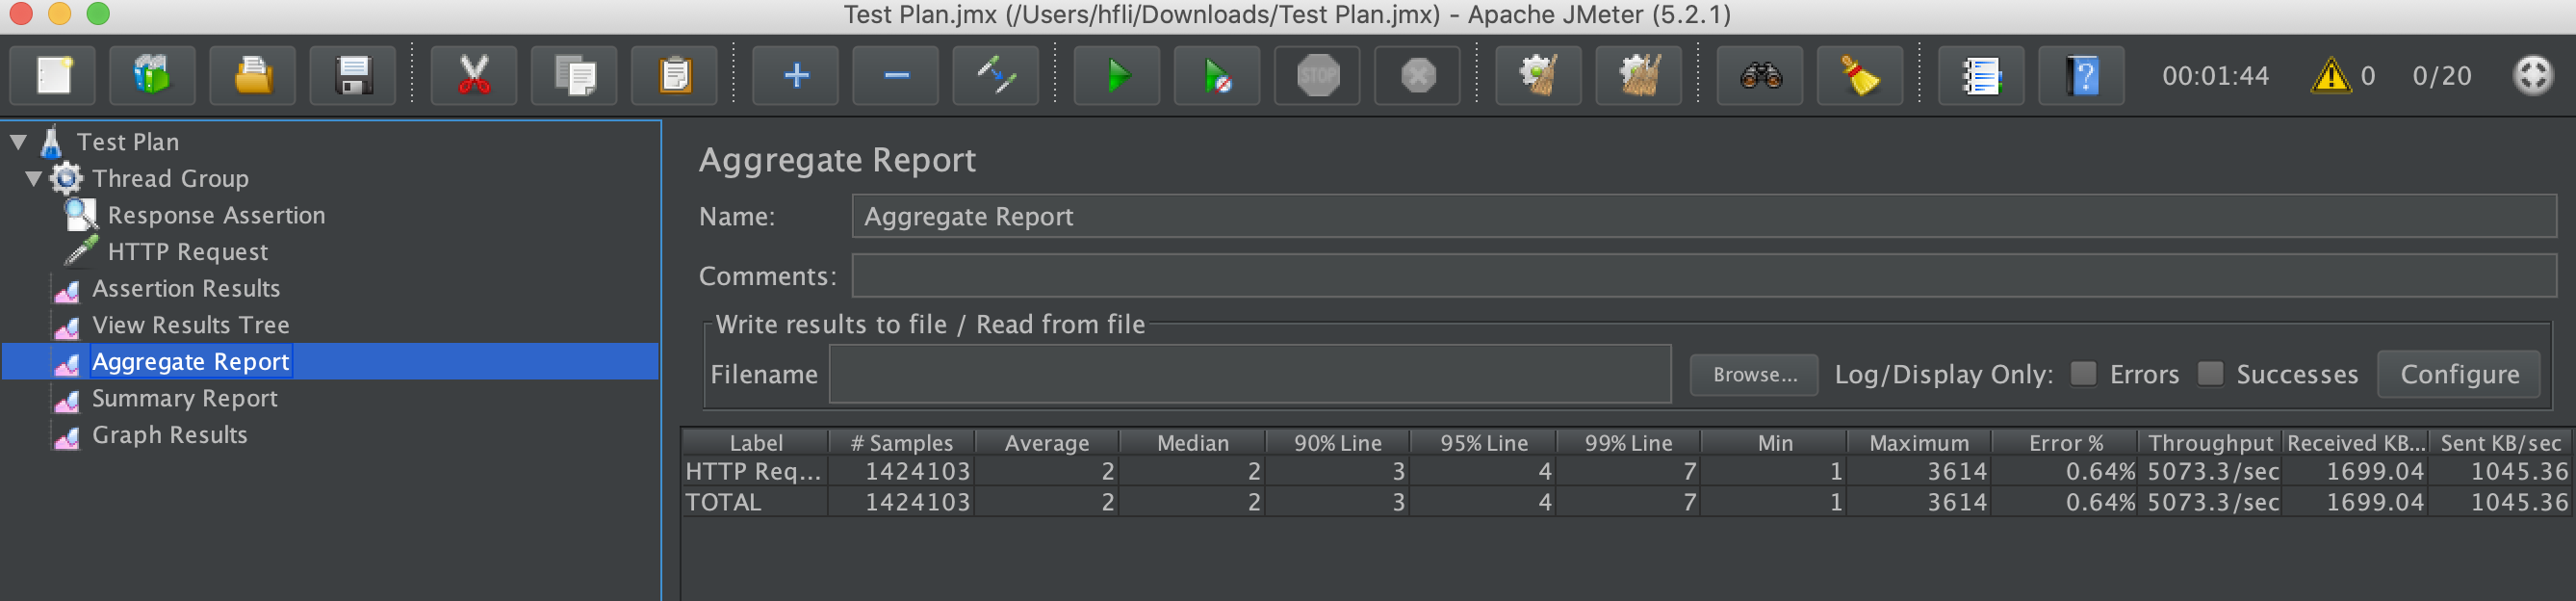
\includegraphics[keepaspectratio,alt={Jmeter}]{images/Jmeter-report.png}}
\caption{Jmeter}
\end{figure}

A few components should be added into the test plan:

\begin{itemize}
\tightlist
\item
  Thread group: to execute a lot of requests parallelly, eg. 20 threads, and using infinite loop
\item
  Http Request sampler: to send post api
\item
  Assertion results: to verify the request, eg. verify the response code should be 200
\item
  Report: eg. Aggregate report to virtualize the result
\end{itemize}

\subsection{Round1: Redis with 128m memory}\label{round1-redis-with-128m-memory}

Let's set the memory limit of redis container to 128m, by using this commands:

\begin{Shaded}
\begin{Highlighting}[]
\ExtensionTok{docker}\NormalTok{ run }\AttributeTok{{-}{-}name}\NormalTok{ redis{-}128 }\DataTypeTok{\textbackslash{}}
           \AttributeTok{{-}d} \DataTypeTok{\textbackslash{}}
           \AttributeTok{{-}p}\NormalTok{ 6381:6379 }\DataTypeTok{\textbackslash{}}
           \AttributeTok{{-}{-}memory}\OperatorTok{=}\StringTok{"128m"} \DataTypeTok{\textbackslash{}}
           \AttributeTok{{-}v}\NormalTok{ /Users/hfli/Downloads/redis{-}test{-}data/redis{-}128:/data }\DataTypeTok{\textbackslash{}}
\NormalTok{           redis redis{-}server}
\end{Highlighting}
\end{Shaded}

Note that the option \texttt{-\/-memory="128m"} sets the memory limitation for redis container, and also we perisit the data into a local volumum so that it will never lose after container restart.

To find the memory usage status of docker container, we can use the \texttt{docker\ stats} command:

\begin{verbatim}
# docker stats
CONTAINER ID        NAME                CPU %               MEM USAGE / LIMIT   MEM %               NET I/O             BLOCK I/O           PIDS
a38d4615af6b        redis-128           0.12%               126.8MiB / 128MiB   99.06%              182MB / 18.6MB      3.08GB / 264MB      6
\end{verbatim}

After successfully started redis, now we are able to use jmeter to test it. Keep running the job, and soon we'll get error in the application:

\begin{Shaded}
\begin{Highlighting}[]
\NormalTok{Servlet.service() for servlet [dispatcherServlet] in context with path [] threw exception [Request processing failed; nested exception is org.springframework.data.redis.RedisSystemException: }
\NormalTok{Error in execution; nested exception is io.lettuce.core.RedisCommandExecutionException: }
\NormalTok{MISCONF Redis is configured to save RDB snapshots, but it is currently not able to persist on disk. Commands that may modify the data set are disabled, because this instance is configured to report errors during writes if RDB snapshotting fails (stop{-}writes{-}on{-}bgsave{-}error option). }
\NormalTok{Please check the Redis logs for details about the RDB error.] with root cause}
\end{Highlighting}
\end{Shaded}

And we can also get some info about redis by using \texttt{info}（or use \texttt{info\ memory} to only get the info related to memory ) and \texttt{dbsize} command in redis-cli:

\begin{verbatim}
# redis-cli
127.0.0.1:6379> info
...
# Memory
used_memory:238777840
used_memory_human:227.72M
used_memory_rss:134189056
used_memory_rss_human:127.97M
used_memory_peak:238777840
used_memory_peak_human:227.72M
used_memory_peak_perc:100.00%
used_memory_overhead:42998602
used_memory_startup:791264
used_memory_dataset:195779238
used_memory_dataset_perc:82.26%
\end{verbatim}

So it has used actually more that 128M!

\begin{verbatim}
127.0.0.1:6379> dbsize
(integer) 843802
\end{verbatim}

Now the redis server is able to start, but it will crash if you try to run \texttt{keys\ *} command.

\subsection{Round2: Redis with 128m memory and maxmemory}\label{round2-redis-with-128m-memory-and-maxmemory}

\begin{Shaded}
\begin{Highlighting}[]
\CommentTok{\# redis.conf}
\ExtensionTok{maxmemory}\NormalTok{ 100mb}
\end{Highlighting}
\end{Shaded}

Add the above maxmemory setting in redis.conf and then start redis by this:

\begin{Shaded}
\begin{Highlighting}[]
\ExtensionTok{docker}\NormalTok{ run }\AttributeTok{{-}v}\NormalTok{ /Users/hfli/Downloads/redis{-}test{-}data/redis{-}128.conf:/usr/local/etc/redis/redis.conf }\DataTypeTok{\textbackslash{}}
           \AttributeTok{{-}{-}name}\NormalTok{ redis{-}128{-}max }\DataTypeTok{\textbackslash{}}
           \AttributeTok{{-}d} \DataTypeTok{\textbackslash{}}
           \AttributeTok{{-}p}\NormalTok{ 6381:6379 }\DataTypeTok{\textbackslash{}}
           \AttributeTok{{-}{-}memory}\OperatorTok{=}\StringTok{"128m"} \DataTypeTok{\textbackslash{}}
           \AttributeTok{{-}v}\NormalTok{ /Users/hfli/Downloads/redis{-}test{-}data/redis{-}128{-}max:/data }\DataTypeTok{\textbackslash{}}
\NormalTok{           redis redis{-}server /usr/local/etc/redis/redis.conf}
\end{Highlighting}
\end{Shaded}

This time we'll still get error when inserted lots of items, but the error message is a little bit different then:

\begin{verbatim}
nested exception is org.springframework.data.redis.RedisSystemException: 
Error in execution; nested exception is io.lettuce.core.RedisCommandExecutionException:
 OOM command not allowed when used memory > 'maxmemory'.] with root cause
\end{verbatim}

That's because the default behavior of redis is that it will return error when memory limit is reached.

\subsection{Round3: Redis with 128m memory and maxmemory and lru}\label{round3-redis-with-128m-memory-and-maxmemory-and-lru}

Try to add one more line to set the lru policy for redis:

\begin{Shaded}
\begin{Highlighting}[]
\CommentTok{\# redis.conf}
\ExtensionTok{maxmemory}\NormalTok{ 100mb}
\ExtensionTok{maxmemory{-}policy}\NormalTok{ allkeys{-}lru}
\end{Highlighting}
\end{Shaded}

Then even if we keep inserting new data into redis, we'll never get some error, because redis will automatically evict the existing items to save memory, that means the \texttt{dbsize} of redis would not be always increcing anymore.

\section{Eviction policy}\label{eviction-policy}

According to the offical document of redis, LRU and LFU(Least Frequently Used) are supported by redis(\textasciitilde4.0). In order to use them first we need to set the memory limit so that redis will use a specified amout of memory for the data set. As shown in the above sections, we can set it in config file or set it thorugh redis-cli at runtime:

\begin{Shaded}
\begin{Highlighting}[]
\ExtensionTok{config}\NormalTok{ set maxmemory 100mb}
\end{Highlighting}
\end{Shaded}

If it's successfully configured we should be able to find it via \texttt{info} command:

\begin{verbatim}
127.0.0.1:6379> info memory
# Memory
...
maxmemory:104857600
maxmemory_human:100.00M
\end{verbatim}

By default is the value \texttt{0} which means no limit at all, and for those running at a 32-bit system there is an implicit memory limit of 3GB.

The evicition policies are listed as bellow:

\begin{itemize}
\tightlist
\item
  \textbf{noeviction}: Return errors
\item
  \textbf{allkeys-lru}: Remove less recently used(LRU) keys first
\item
  \textbf{volatile-lru}: Only remove LRU keys that has expire set
\item
  \textbf{allkeys-random}: Randomly remove keys
\item
  \textbf{volatile-random}: Randomly remove keys that has expire set
\item
  \textbf{volatile-ttl}: Evict keys with expire set and keys has shorter time to live(TTL) will be removed firstly
\item
  \textbf{volatile-lfu}: Remove less frequently used(LFU) keys first
\item
  \textbf{allkeys-lfu}: Remove LFU keys that has expire set
\end{itemize}

For volatile-lru, volatile-lfu, volatile-random and volatile-ttl policies, it's possible that no keys are available to be removed, then redis will behave like noeviction(ie. throw error).

\subsection{How to choose policy}\label{how-to-choose-policy}

Generally LFU will be better than LRU, try to think that some items recently accessed but is actually almost never accessed in the future, if you use LRU then there is a risk that items get higher chance to be requested in the future will be evicted, while LFU does not have such a problem.

In short, follow these rules to choose the evict policy:

\begin{itemize}
\tightlist
\item
  \textbf{allkeys-lru}: If you expect that some elements will be accessed far more often than the rest, choose it. And if you're not sure, this is also the suggested option for you.
\item
  \textbf{allkeys-random}: If you'd prefer that all elements have the same chance to be accessed, use it.
\item
  \textbf{volatile-ttl}: If you wish to evict keys according to ttl
\item
  \textbf{volatile-lru/volatile-random}: If you use the same redis for both persistent keys and caching, \emph{BUT} usually in this case it's suggested to run two seperate instance of redis.
\end{itemize}

\subsection{Controll LRU precision}\label{controll-lru-precision}

The redis LRU algorithm is an approxmimated LRU algorithm, the reason behind is that use true LRU algorithm will cost more memory, while the approximation is virtually equivalent (good enough) for the application using redis.

And you're able to tune the precision of LRU by:

\begin{Shaded}
\begin{Highlighting}[]
\ExtensionTok{maxmemory{-}samples}\NormalTok{ 5}
\end{Highlighting}
\end{Shaded}

The larger value you use, the more approximated you will get, but also with more CPU usage.

\begin{verbatim}
maxmemory_human:0B
maxmemory_policy:noeviction
\end{verbatim}


\end{document}
